\section{Results}
The algorithm was tested with different audio samples. The most important tests were done with anechoic samples of a single violin player, as this was closest to the original purpose. We also tested the algorithm with samples of recorded electric guitar, and an already heavily processed piece of music. Different parameter values for the algorithm were also tested.

Figure~\ref{fig:dryspec} shows the spectrogram of an uneffected, anechoic violin recording. The partials are clear and the vibrato of the player is also easy to see, particularly around the $2.5s$ time point
\begin{figure}[ht]
\centering
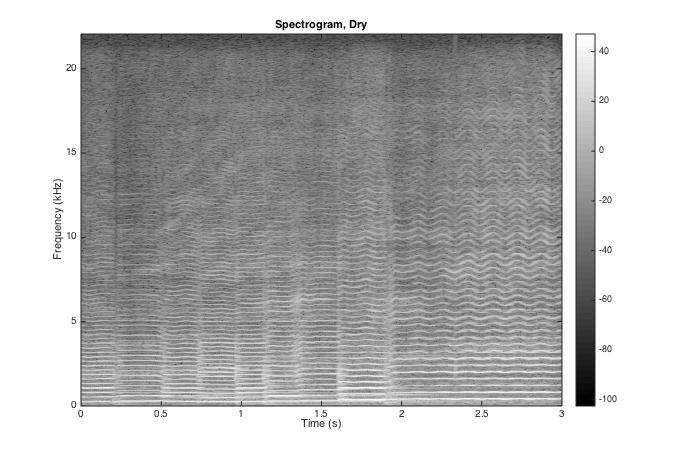
\includegraphics[width=\textwidth]{dry_spec.png}
\caption{Spectrogram of dry signal.}
\label{fig:dryspec}
\end{figure}

Figure~\ref{fig:effspec} shows the spectrogram of the same sample as figure~\ref{fig:dryspec}, but this time passed through the Warm Chorus algorithm. Though the partials are still some what visible, the spectrogram is now more blurry and the vibrato of the original recordings appears to be masked by the effect.
\begin{figure}[ht]
\centering
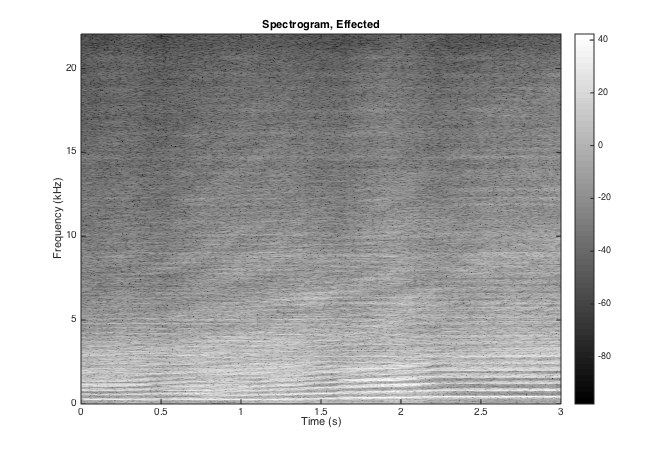
\includegraphics[width=\textwidth]{effected_spec.png}
\caption{Spectrogram of effected signal.}
\label{fig:effspec}
\end{figure}

The blurryness is explained by two factors. Firstly, as is also audible, the algorithm gives the input a reverberated quality due to the reasonably long delays. This blurs the spectrogram in the horisontal direction Secondly, the harmonisers spread the frequency content, which blurs the spectrogram in the vertical direction.

The algorithm's output has no obvious periodic pulse. The output gives the impression of many players playing the same thing in a space. The spaciousness seems inseparable from the impression of a section of players.

When compared with a generic chorus algorithm, the Warm Chorus is much more convincing and realistic. However, the generic chorus has a distinct sound of its own.

When using some extreme settings, the Warm Chorus algorithm may produce quite unpleasant results. After some point, the detuning of the input makes the output sound audibly out-of-tune. Similarly, too much simulated distance between the players results in losing temporal accuracy.
